% This is added to allow editing only this part of the document
\documentclass[A4,12pt,oneside]{article}
%A4,12pt,titlepage,oneside,final

% list of packages
\usepackage[a4paper,left=2cm,right=2cm,top=2cm,bottom=2cm]{geometry} % document size

\usepackage[utf8]{inputenc}
\usepackage[T2A]{fontenc} %russian language encoding

\usepackage{textcomp}
\usepackage{lmodern}
\usepackage{amsmath}
\usepackage{hyperref}
\usepackage{xcolor}
\usepackage{graphicx}
\usepackage{listings}
\usepackage{listingsutf8}
\usepackage{dcolumn}   % needed for some tables
\usepackage{bm}        
\usepackage{amssymb} 
\usepackage{fancyvrb}
\usepackage{fvextra}
\usepackage{array}
\usepackage{multicol}
\usepackage{setspace}

%russian language support
\usepackage[english,russian]{babel}
%starts at the last language on the list
%select language switches the language


\makeatletter


%\graphicspath{{figs/error_en}} % Directory in which figures are stored


%
% list of custom commands
\newcommand{\be}{\begin{equation}}
\newcommand{\ee}{\end{equation}}
\newcommand{\bea}{\begin{eqnarray}}
\newcommand{\eea}{\end{eqnarray}}
\renewcommand{\(}{\left(}
\renewcommand{\)}{\right)}
\newcommand{\citeph}{\textcolor{red}{[ref] }}

\newcommand{\rut}{\selectlanguage{russian}}
\newcommand{\ent}{\selectlanguage{english}}


%\newcommand{\be}{\begin{equation}}
%\rnc{\d}{\mathrm{d}}
%\nc{\D}{\partial}
%\nc{\nn}{\nonumber}
%\rnc{\inf}{\infty}
%\nc{\vphi}{\varphi}
%\nc{\half}{\frac{1}{2}}


% color commands are used to highlight text temporarily, for editing
\newcommand{\nadd}[1]{\textcolor{magenta}{#1}}
\newcommand{\ncomm}[1]{\textcolor{magenta}{\bf{[#1]}}}
\renewcommand{\Re}{\mathrm{Re}}
\renewcommand{\Im}{\mathrm{Im}}




\makeatother

\begin{document}


\section{Решение начальных задач}

%Since the equation of analysis in this work is nonlinear, the the solutions are analyzed by numerical analysis. There are techniques for finding an approximate solution analytically, but they only provide limited insight in this case. The solution for the ODE shows a similar structure, but with a frequency shift dependent on the nonlinearity coefficient and the initial derivative of the wave function.

Поскольку уравнение, анализируемое в этой работе, является нелинейным, решения исследованы с помощью численными методами. Существуют методы нахождения приближенного решения аналитическим путем, но в данном случае они дают лишь ограниченное понимание. Решения начальной задачи для нелинейного уравнения Шредингера показывают аналогичную структуру решения, но со смещением частот, зависящим от коэффициента нелинейности и начальной производной волновой функции.

\subsection{Численный анализ}

%We proceed with analysis of the nonlinear time-independent Schrödinger equation
Переходим к анализу нелинейного стационарного уравнения Шредингера,
\begin{equation}\label{eqn:schrod}
\hat{H} \psi = k^2 \psi = \left( i \frac{d}{dx} + \frac{\pi BR}{\Phi_0} \right)^2 \psi + \mu \frac{m_e}{\left|e\right|\hbar} \left|\psi\right|^2 \psi,
\end{equation}
%subject to the boundary condition $\psi\left(0\right) = \psi\left(2 \pi R\right)$. As a reminder, the choice of $\psi\left(0\right)$ is irrelevant, since if $\mu$ is redefined as $\mu_{eff} = \mu_{true}\left|\psi\left(0\right)\right|^2$, changes to $\psi\left(0\right)$ leave the Schrödinger equation unchanged, provided one remembers to properly rescale $\mu$. The boundary condition is completely unchanged by this transformation. So we can freely define $\psi\left(0\right) = 1$ and work with $\mu_{eff}$. It is also worth noticing that with this definition, $\mu_{eff}$ is the same for all rings if $\mu$ as defined here is the same for all rings, since $\psi\left(0\right)$ is the same for all rings.
при соблюдении граничного условия $\psi\left(0\right) = \psi\left(2 \pi R\right)$. Напомним, что выбор значения $\psi\left(0\right)$ не имеет значения, поскольку, если $\mu$ переопределено как $\mu_{eff} = \mu_{true}\left|\psi\left(0\right)\right|^2$, изменение $\psi\left(0\right)$ оставляет уравнение Шредингера неизменным, при условии, что $\mu$ правильно масштабировано. Граничные условия при этом преобразовании полностью не меняется. Таким образом, можно свободно определять $\psi\left(0\right) = 1$ и работать с $\mu_{eff}$. Также стоит отметить, что при таком определении $\mu_{eff}$ одинаково для всех колец, если $\mu=\frac{\mu_{eff}}{\left|\psi\left(0\right)\right|^2}$ одинаково для всех колец, так как $\psi\left(0\right)$ одинаково для всех колец.

Численный анализ работает с начальными задачами. Нужно решить уравнение Шредингера, начиная с момента времени (или, скорее, положения в данном случае) $ t = 0$, и вычислять вперед во времени с помощью системы дифференциальных уравнений первого порядка. Это означает, что требуется выполнить два преобразования уравнения Шредингера. Более простым из двух является простое преобразование переменных. Мы определяем независимую переменную $t = x$ и новую зависимую переменную $y = \frac{d\psi}{dt}$. Уравнение \ref{eqn:schrod}, переписанное как система обыкновенных дифференциальных уравнений в стандартной форме, таким образом, принимает вид,
%Numerical analysis works with an initial value problem. One needs to solve the Schrodinger equation starting from a time (or rather position in this case) $t=0$, and evolve forward in time with a system of first order differential equations. This means that one is required to perform two transformations of the Schrodinger equation. The easier of the two is a simple transformation of variables. We define the independent variable $t = x$ a new dependent variable $y = \frac{d\psi}{dt}$. Equation \ref{eqn:schrod} rewritten as a system of ordinary differential equations in standard form thus takes the form,
\begin{align}
\frac{d\psi}{dt} & = y\\
\frac{dy}{dt} & = 2 i \frac{\pi BR}{\Phi_0} y + \frac{\pi^2 B^2R^2}{\Phi^2_0}  \psi + \mu \frac{m_e}{\left|e\right|\hbar} \left|\psi\right|^2 \psi -k^2 \psi,
\end{align} 
где для линейного случая $\mu = 0$. Эта стандартная форма обыкновенных дифференциальных уравнений, которая используется в стандартных алгоритмах численного анализа, но только в качестве начальной задачи. Чтобы решить краевую задачу, необходимо найти значение $\frac{d\psi}{dx}\left(0\right)$, которое задает решение этого уравнения, соответствующее граничному условию.
%where, for the linear case, $\mu = 0$. This standard form of the ODE is now usable with standard numerical analysis algorithms, but only as an initial value problem. To solve the boundary value problem, one needs to find the values of $\frac{d\psi}{dx}\left(0\right)$ which provide a solution to this equation satisfying the boundary condition. 

Существует множество алгоритмов для решения обыкновенных дифференциальных уравнений. Они, как правило, более разумны, чем просто выполнение равных шагов по времени $dt$ и использование производной от предыдущего шага для оценки значений зависимых переменных на следующем шаге с помощью $dx = \frac{dx}{dt}dt$, где $x\left(t + dt\right) = dx\left(t\right) * x\left(t\right)$ и $\frac{dx}{dt} = \frac{dx}{dt} \left(t\right)$. 
Стандартные алгоритмы происходят из семейства, названного Рунге-Кутта в честь их первооткрывателей. Различные алгоритмы Рунге-Кутты различаются тем, как они берут и взвешивают промежуточные точки, выбираемые на основе соответствия и минимизации количества вычислительных шагов и ошибки, а также тем, следует ли использовать второй, более точный алгоритм для оценки идеального размера шага при заданном допуске, оценивая ошибку на основе разницы между двумя алгоритмы Рунге-Кутты. Точная форма этих двух алгоритмов выбрана для повторного использования вычислений, чтобы предотвратить удвоение объёма требуемых вычислений при выполнении интегрирования дважды. Простой алгоритм, описанный раньше, также считается алгоритмом Рунге-Кутты и называется методом Эйлера. \citeph
%Algorithms for solving ordinary differential equations are numerous. They are typically more intelligent than just taking even time steps $dt$ and using the derivative of the previous step to estimate the values of the dependent variables in the next step by means of $dx = \frac{dx}{dt}dt$, where $x\left(t + dt\right) = dx\left(t\right) * x\left(t\right)$, and $\frac{dx}{dt} = \frac{dx}{dt} \left(t\right)$. 
%The standard algorithms come from a family called Runge-Kutta (RK), after their discoverers. Various Runge-Kutta algorithms vary in how they take and weigh intermediary points, selected based on consistency and minimization of computational steps and error, and whether or not to use a second, more precise algorithm to estimate ideal step size for a given tolerance, estimating the error based on the difference between the two RK algorithms. The exact form of these two algorithms are chosen to reuse calculations, thus preventing a doubling of the required calculations when performing the integration twice. The simple algorithm described here is also considered an RK algorithm, by the name of the Euler method. \citeph

Существует несколько стандартных методов решения краевых задач, но все они начинаются с решения начальной задачи. Два наиболее распространенных метода -- это метод стрельбы и метод конечных разностей. Метод стрельбы предполагает простую логику -- человек угадывает решение, пока не найдет то, которое работает. На практике это работает аналогично большинству итерационных алгоритмов -- человек начинает с одной или двух разумных догадок и продвигается к решению. Метод конечных разностей вместо этого работает, помещая систему в решетку и решая от обоих направлений. \citeph В этом анализе не используется ни один из вариантов, поскольку модели смещения вольных чисел, найденные в решениях начальной задачи, достаточно хороши, чтобы соответствовать граничным условиям в пределах допустимого, в то время как ошибка в численном алгоритме означает, что решения, найденные им, не будут полезны без вычитания ошибки.
%There are several standard techniques for solving boundary value problems, but they all start with solving the initial value problem. The two most common techniques are shooting and finite difference methods. Shooting involves straightforward logic -- one guesses the solution until they find one which works. In practice this works similarly to most iterative algorithms -- one starts with one or two intelligent guesses and works their way towards the solution. Finite difference methods instead work by putting the system on a lattice, and solving in both directions. \citeph  In this analysis neither variant will be used, as the models found for solutions to the initial value problem are good enough to match both sides within tolerance, while error in the numerical algorithm means that solutions provided by it will not be useful without subtracting the error. 

Чтобы определить, как наилучшим образом подойти к решению краевой задачи, этот анализ начинается с решения начальной задачи для заданных значений $\frac{d\psi}{dx}$. В предположении, что решение должно быть близко к линейному случаю, мы начинаем с выбора $\frac {d\psi}{dx}$, чтобы оно соответствовало решению краевой задачи для линейного случая (с $\mu = 0$), \citeph
%In order to determine how to best approach the boundary value problem, this analysis starts with solving the initial value problem for given values of $\frac{d\psi}{dx}$. Under the assumption that the solution should be close to the linear case, we start by choosing $\frac{d\psi}{dx}$ to conform to the solution of the boundary value problem for the linear case (with $\mu = 0$). This is given by \citeph
\begin{align}\label{eqn:linbvp1}
\frac{d\psi_j}{dx}\left(0\right) &= i \left(a_j \left(k_0 + M_0\right) + b_j \left(-k_0 + M_0\right)\right)\\
a_j &= \frac{1- e^{i\left(-k_0 + M_0\right) 2\pi R_j}}{2 i e^{2 i \pi M_0 R_j} \sin\left(2\pi k_0 R_j\right)}\\
b_j &= \frac{-1 + e^{i\left(k_0 + M_0\right) 2\pi R_j}}{2 i e^{2 i \pi M_0 R_j} \sin\left(2\pi k_0 R_j\right)}\label{eqn:linbvp2}
\end{align}
Выбираем $k = k_ {Fermi, Au}$, $R = 8 \times 10^{-7}$ м, $B = 0,5\, B_{max}$ и $\mu = 10^{-6}$.
%We choose $k = k_{Fermi, Au}$, $R = 8 \times 10^{-7}$ m, $B = 6.5 \times 10^{-3}$ T, and $\mu = 10^{-6}$. 

Сразу появляется проблема. Используемое значение $k_{Fermi, Au} = 1,20 \times 10^{10}$ м$^{-1}$ \citeph недостаточно точно для нахождения ненулевых значений $\sin\left(2\pi k R\right)$, где $kR = 1,20 \times 10^{10}\, *\, 0.9 \times 10^{-6} = 1.20 * 0.9 \times 10^{4}$. Когда $\sin\left(2\pi k R_j\right)=0$, решения краевой задачи для линейного уравнения Шредингера становятся неоднозначными, поскольку колебания точно помещаются в кольцо, и выбор точки в колебаниях, в которой производная была бы прерывистой, становится ненужным. Чтобы решить эту проблему, был добавлен дифференциал $dk$ в пределах неопределенности значения $k$, так что $k = k_{Fermi, Au} + dk$. Чтобы $k$ не попадало на границу, уравнение для $k$ в коде имеет вид
%We immediately encounter a problem. The value $k_{Fermi, Au} = 1.20 \times 10^{10} \, \mathrm{m}^{-1}$ \citeph  which we are using is not precise enough for finding non-zero values of $\sin\left(2\pi k R\right)$, with $kR = 1.20 \times 10^{10}\, *\, 0.9 \times 10^{-6} = 1.20 * 0.9 \times 10^{4}$. When $\sin\left(2\pi k R_j\right)=0$ the boundary value problem solutions become ambiguous for the linear Schrodinger equation, as the oscillations exactly fit in the ring, and choosing a point in the oscillations for the derivative to be discontinuous becomes unnecessary. In order to solve this problem, a differential $dk$ within the limits of the uncertainty in the value of $k$ was added, so $k = k_{Fermi, Au} + dk$. So that $k$ doesn't fall on a boundary, the equation for $k$ in the code is
\begin{equation}\label{eqn:fullk}
k = k0 + \frac{dk}{2 R_{max}}.
\end{equation}
Здесь $k0 = k_{Fermi, Au}$ и $dk$ выбраны так, чтобы они имели значения $(0, 1)$. Эта настройка позволяет избежать неоднозначности в решении линейного уравнения Шредингера. Теперь можно перейти к построению графика этих решений. Когда $k0 = 1,20 \times 10^{10}$ м$^{-1}$, $dk = 0,5$, $R = 0,8\, R_{max} = 8 \times 10^{-7}$ м, $B = 0,5\, B_{max}$, $\mu = 10^{-6}$ и $\frac{d\psi}{dx}\left(0\right)$ равно тому, которое решает краевую задачу для линейного уравнения Шредингера (уравнения \ref{eqn:linbvp1}-\ref{eqn:linbvp2}), решения выглядят так, как показано на рисунке \ref{fig:linbvp}.
%Here, $k0 = k_{Fermi, Au}$, and $dk$ is chosen to have values $(0, 1)$. This setup avoids ambiguity in the solution for the linear Schrodinger equation. One can now proceed to plot these solutions. For values of $k0 = 1.20 \times 10^{10}$ $\mathrm{m}^{-1}$,  $dk = 0.5$, $R = 0.8\, R_{max} = 8 \times 10^{-7} \, \mathrm{m}$,  $B = 0.5\, B_{max} = 6.5 \times 10^{-3}\, \mathrm{T}$, $\mu = 10^{-6}$ and $\frac{d\psi}{dx}\left(0\right)$ set to that which solves the boundary value problem for the linear case (Equations \ref{eqn:linbvp1}-\ref{eqn:linbvp2}), the solutions look like those shown in Figure \ref{fig:linbvp}.
\vspace{-1.3cm}

\begin{center}
\begin{figure}
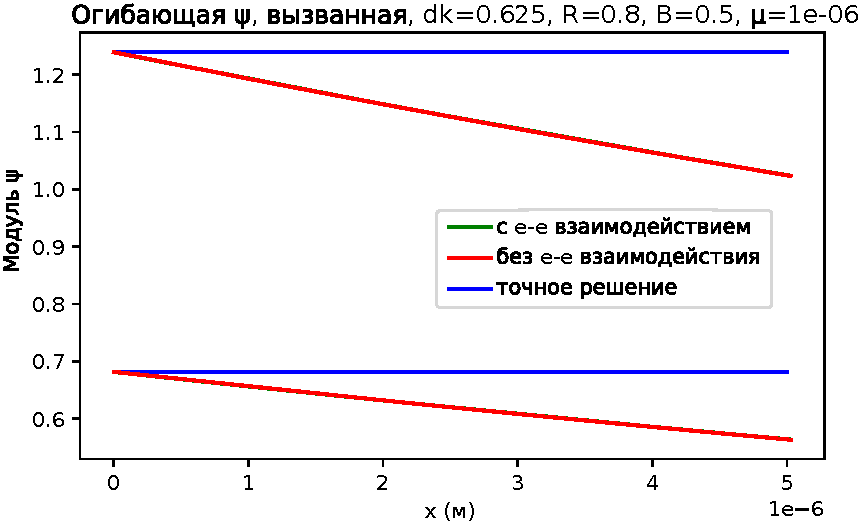
\includegraphics[width=0.4\paperwidth]{figs/error_ru/plot_abs_env_v2}
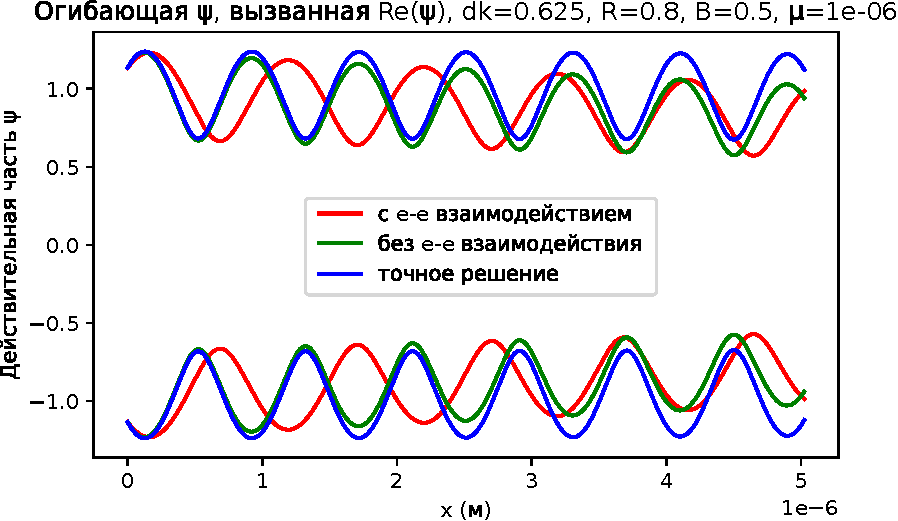
\includegraphics[width=0.4\paperwidth]{figs/error_ru/realEnv1}

\includegraphics[width=0.4\paperwidth]{figs/error_ru/plot_abs_full}

\includegraphics[width=0.4\paperwidth]{figs/error_ru/plot_real_full}
\caption{\label{fig:linbvp}
На рисунках показана вольная функция $\psi\left(x\right)$, решающего начальную задачу, когда $k0 = 1,20 \times 10^{10}$ м$^{-1}$, $dk = 0,5$, $R = 0,8\, R_{max} = 8 \times 10^{-7}$ м, $B = 0,5\, B_{max}$, $\mu = 10^{-6}$ и $\frac{d\psi}{dx}\left(0\right)$ равно тому, которое решает краевую задачу для линейного уравнения Шредингера.\\
\textbf{Вверху:} Огибающая быстрых колебаний модуля (слева) и действительной части (справа) волновой функции $\psi\left(x\right)$. Синие кривые показывают пределы известного точного решения линейного уравнения Шредингера. Зеленые и красные кривые показывают результаты численного интегрирования для линейного и нелинейного уравнений Шредингера в таком порядке. На первом рисунке зеленая кривая скрыта за красной кривой и поэтому может быть не видна. \\
\textbf{Внизу:} График модуля (слева) и действительной части (справа) волновой функции $\psi\left(x\right)$, которая представляет собой линейное решение, вычисленное по формуле, а не численное интегрирование. Хотя кажется, что графики содержат заштрихованную область, это всего лишь результат того, что ширина линии больше периода колебаний. Эти графики были намеренно сохранены в растровом графическом формате, а не в виде векторной графики, так как в противном случае графика загружалась бы медленно из-за большого количества точек и вычислений.
%\textbf{Top:} Curves of the maximum extent of the fast oscillations of the absolute value (left) and real part (right) of the wave function $\psi\left(x\right)$. The blue curves show the limits of the known exact solution to the linear Schrodinger equation. The green and red curves show the results of numerical integration for the linear and nonlinear Schrodinger equations, respectively. In the first image, the green curve is hidden behind the red curve, and therefore may not be visible. \\
%\textbf{Bottom:} Graph of the absolute value (left) and real part (right) of the wave function $\psi\left(x\right)$ which solves the linear solution, calculated from the formula, not numerical integration. While the graphs appear to contain a shaded region, this is just the result of the line width being thicker than the period of oscillation. These graphs have been purposefully saved in a raster graphic format, not as a vector graphic, as otherwise the graphics would load slowly due to the large number of points and calculations.
}
\end{figure}
\end{center}

Здесь кривые на рисунках обозначают локальный минимум или максимум значений $\Re\left(\psi\right)$ или $\left|\psi\right|$, зависимо от кривой. Кривая основана на триггере, настроенном в алгоритме решения обыкновенных дифференциальных уравнений, который находит точки в решении, для которых задана производная, либо $\frac{d\left|\psi\right|}{dx}$, либо $\frac{d\Re\left(\psi\right)}{dx}$, достигает нуля. Без этого всё пространство между двумя изображенными линиями было бы заполнено точками, затеняющими всю область, как видно на двух нижних графиках, что затрудняло бы просмотр кривых и значительно замедляло бы загрузку графики, если она использует векторный формат. По-видимому, решения колеблются чрезвычайно быстро, с быстрыми колебаниями во всем диапазоне около $2000$. На рисунке \ref{fig:beginfo} показан пример $\Re\left(\psi\right)$ и $\left|\psi\right|$ для первых нескольких таких колебаний.
%Here the curves in the figures designate the greatest extent of the oscillations for both the $\Re\left(\psi\right)$ and $\left|\psi\right|$ values. The curve is based on a trigger set up in the ODE solving algorithm, which finds the points on the solution for which the given derivative, either $\frac{d\left|\psi\right|}{dx}$ or $\frac{d\Re\left(\psi\right)}{dx}$, reaches zero. Without this, the whole space between the two depicted lines would be full of points, shading the entire region, as seen in the two lower plots, making the curves difficult to see, and significantly slowing down loading the graphics if it uses a vector format. Apparently, the solutions oscillate extremely quickly, with around $10^4$ fast oscillations in the entire range. Figure \ref{fig:beginfo} shows an example of $\Re\left(\psi\right)$ and $\left|\psi\right|$ for the first several such oscillations.
\vspace{-1.2cm}
\begin{center}
\begin{figure}
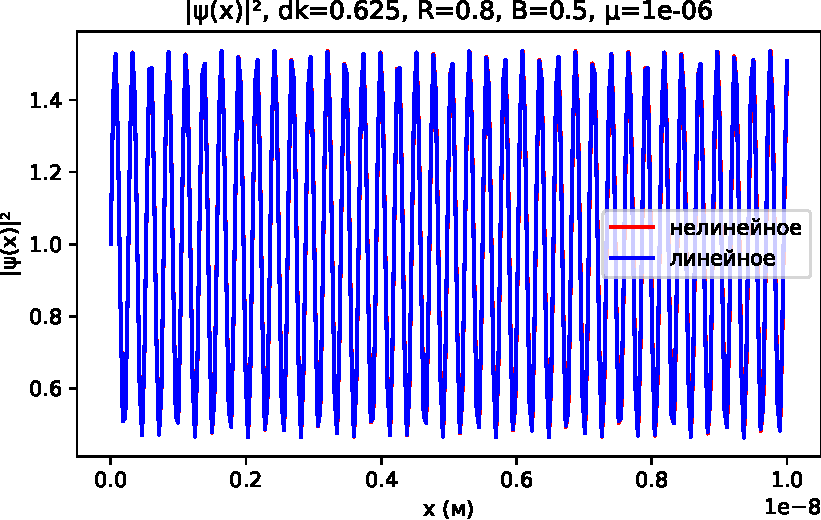
\includegraphics[width=0.4\paperwidth]{figs/error_ru/fastoscabs}
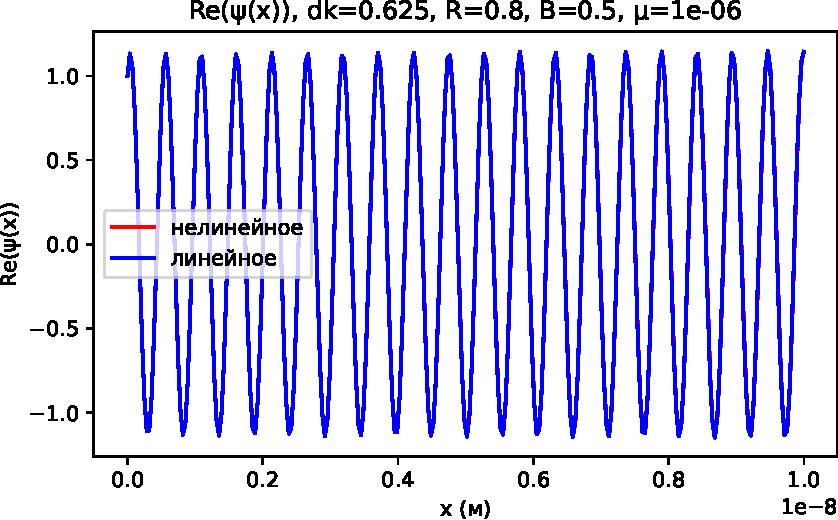
\includegraphics[width=0.4\paperwidth]{figs/error_ru/fastoscre}
\caption{\label{fig:beginfo}
На рисунках показаны первые несколько быстрых колебаний $\psi\left(x\right)$, решающего начальную задачу, когда $k0 = 1,20 \times 10^{10}$ м$^{-1}$, $dk = 0,5$, $R = 0,8\, R_{max} = 8 \times 10^{-7}$ м, $B = 0,5\, B_{max}$, $\mu = 10^{-6}$ и $\frac{d\psi}{dx}\left(0\right)$ равно тому, которое решает краевую задачу для линейного уравнения Шредингера. Левый график показывает $|\psi|^2$, в то время как правый график показывает $\Re\left(\psi\right)$, которые вместе показывают полную информацию о $\psi$. В обоих случаях кривая для нелинейного уравнения Шредингера (красная) скрыта за кривой для линейного уравнения Шредингера (синяя).
%Graph of the first few fast oscillations of $\psi\left(x\right)$ The left graph shows $|\psi|^2$, while the right graph shows $\Re\left(\psi\right)$, which together show complete information of $\psi$. In both cases, the curve for the nonlinear Schrodinger equation (red) is hidden behind the curve for the linear Schrodinger equation (blue). 
}
\end{figure}
\end{center}

\subsection{Ошибка}
На рисунке \ref{fig:linbvp} также показана ещё проблема с решениями. Известное точное решение и численное решение линейного уравнения Шредингера не совпадают. 
С самого начала существовала сложность, небольшая численная погрешность в сумме с многочисленными колебаниями быстрых колебаний стала чем-то значительным.
%Figure \ref{fig:linbvp} also reveals another issue with the solutions. The known exact solution and the numerical solution to the linear Schrodinger equation do not agree. 
%From the beginning there was a complication, the small numerical error adds up to something significant over the numerous oscillations of the fast oscillations.

%For gold, the Fermi wave number I found is $k = 1.20 \times 10^{10}$. This corresponds to a speed of 
%\begin{equation}
%v = \frac{\hbar k}{m} \approx 0.0043 c
%\end{equation}
%Our electrons in their ground state are traveling quite fast within the metal. This is actually part of the requirement for ballistic motion -- the highest energy electron in the ground state of the metal is traveling at significant speed relative to the small radius. An approximation without interaction is good. 

Одним из следствий большого волнового числа Ферми для проводников является то, что существует множество быстрых колебаний ($2000$) по сравнению с медленными колебаниями, вызванными магнитным полем. С математической точки зрения это удобно. Можно смоделировать два типа колебаний отдельно, причем быстрые колебания имеют незначительное изменение амплитуды в течение короткого периода времени, в то время как медленные колебания можно легко увидеть, выбрав точек с разностью их значения, кратные периоду быстрых колебаний. С точки зрения численных методов это проблема. Это означает, что если для каждого колебания существует похожая погрешность, то эта погрешность должна быть умножена на $2000$. Кажущаяся незначительная ошибка скрывает весь сигнал. Результат в этом случае очевиден, поскольку амплитуда быстро убывает, как было видно на рисунке \ref{fig:linbvp}.
%One of the consequences of the large Fermi wave number for conductors is that there are numerous fast oscillations ($10^4$) when compared to the slow oscillations caused by the magnetic field. From a mathematical standpoint, this is convenient. One can model the two types of oscillations separately, with the fast oscillations having negligible variation in amplitude over a short time-frame relevant to them, while the slow oscillations can easily be seen by sampling at differences which are multiples of the period of fast oscillations. From a numerical standpoint, this is a problem. It means that if there is a constant error term from each oscillation, this error must be multiplied by $10^4$. Seemingly insignificant error now hides all of the signal. The result is obvious in this case, as the amplitude rapidly decreases, as was seen in Figure \ref{fig:linbvp}. 
 
%Figure \ref{fig:errAbs} shows another view of this error. Seen here are the curves produced by plotting points when the fast oscillations should reach their maxima, according to our estimates for period. For the exact case, the period of oscillations is given by $\frac{2 \pi}{k}$. Since the produced curve oscillates between a minimum and maximum, this period is incorrect. We can instead estimate the period of oscillations by averaging the half-period of the first several oscillations. (This is the half period, since it is the period of $\left|\psi\right|^2$, which oscillates twice as fast as $\psi$ for a sinusoidal function.) The results are seen in the next two graphs of Figure \ref{fig:errAbs}.
\vspace{-1.2cm}
\begin{center}
\begin{figure}
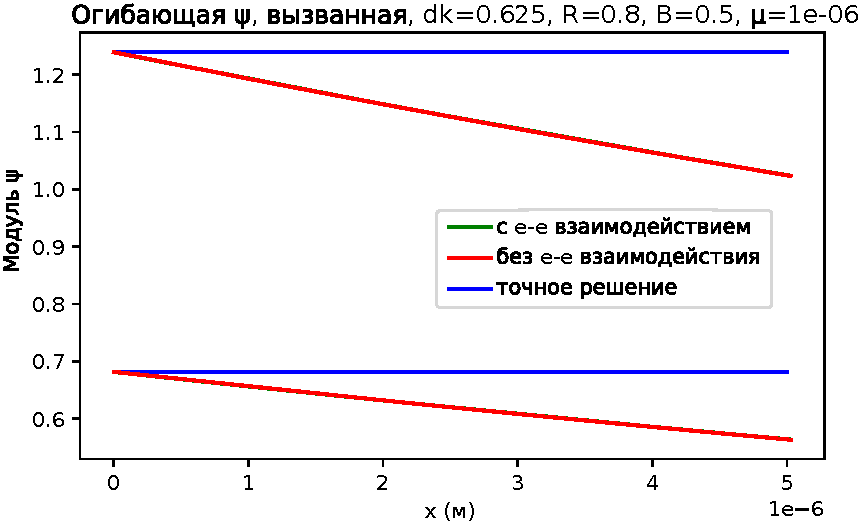
\includegraphics[width=0.4\paperwidth]{figs/error_ru/plot_abs_env_v2}
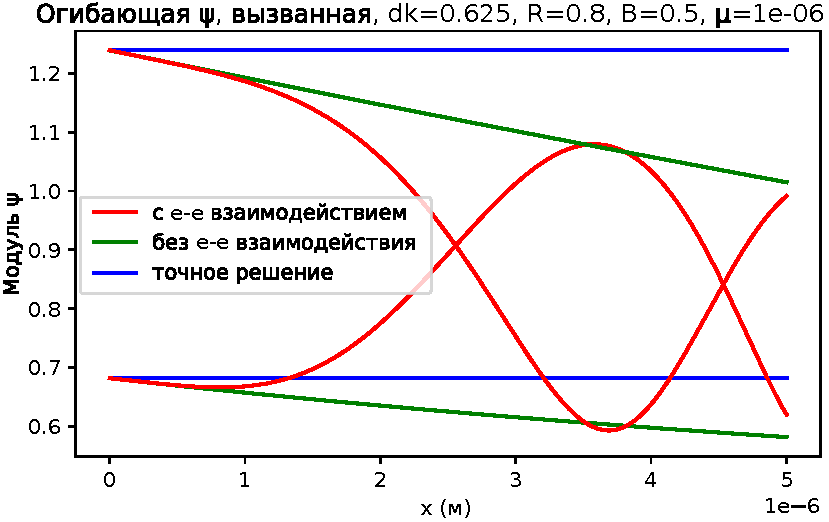
\includegraphics[width=0.4\paperwidth]{figs/error_ru/plot_abs_env5}

\caption{\label{fig:errAbs}
На рисунках показана вольная функция $\psi\left(x\right)$, решающего начальную задачу, когда $k0 = 1,20 \times 10^{10}$ м$^{-1}$, $dk = 0,5$, $R = 0,8\, R_{max} = 8 \times 10^{-7}$ м, $B = 0,5\, B_{max}$, $\mu = 10^{-6}$ и $\frac{d\psi}{dx}\left(0\right)$ равно тому, которое решает краевую задачу для линейного уравнения Шредингера.\\
Слева: График огибающей быстрых колебаниях модуля $\psi$, полученной в результате численных решений линейного (зеленого) и нелинейного (красного) уравнений Шредингера. Огибающая определяется триггером в процессе интегрирования, возвращающим все случаи, когда $\frac{d|\psi|}{dx} = 0$. Зеленая кривая полностью скрыта за красной кривой на этом графике, и этот факт может быть виден, а может и не быть виден. \\
Справа: График того, какой должна быть огибающая, образованная быстрыми колебаниями модуля $\psi$, на основе периода быстрых колебаниях $T_{fast}$, полученного из вычисленного точного значения $T_{fast}$ в линейном случае (зеленый) и оцененного по первым 20 быстрым колебаниям для нелинейного случая (красный). Зеленая линия отклоняется от правильной огибающей из-за небольшой ошибки в периоде, отмечая меньший, чем требуется, участок графика. Красная линия показывает ошибку периода, зависящую от положения, так как у кривых, которые должны быть огибающей, видны асимметричные колебания, а верхняя и нижняя границы пересекаются и временно меняются местами.
%Left: Graph of the envelope formed by the fast oscillations of the absolute value of $\psi$ formed by the numerical solutions to the linear (green) and nonlinear (red) Schrodinger equations. The envelope is determined by a trigger in the integration process, returning all cases when $\frac{d|\psi|}{dx} = 0$. The green curve is completely hidden behind the red curve in this graph, a fact which may or may not be visible. \\
%Right: Graph of what should be the envelope formed by the fast oscillations of the absolute value of $\psi$ based on values of $T_{fast}$ given by the calculated exact value of $T_{fast}$ in the linear case (green) and the value of $T_{fast}$ estimated by the first 20 fast oscillations for the nonlinear case (red). The green line deviates from the correct envelope due to a small error in the period, marking off a smaller than required section of the graph. The red line shows a larger, position dependent, error in the period, as an asymmetric oscillation is visible in what should be the envelope, and the upper and lower bounds cross and switch places temporarily. 
}
\end{figure}
\end{center}

И ещё проблему можно увидеть на рисунке \ref{fig:errAbs}. Период не соответствует ожидаемому. Это известно потому, что выборка волновой функции с шагами, кратными ожидаемому периоду колебаний, не соответствует огибающей этих колебаний. Когда период для решения линейного уравнения Шредингера определяется как известное решение, можно увидеть, что результирующая кривая не совсем совпадает с огибающей.
%Another issue can be seen in Figure \ref{fig:errAbs}. The period is not what is expected. This is known because sampling the wave function with steps taken as multiples of the expected period of oscillations fails to follow the envelope of those oscillations. When the period for solution to the linear Schrodinger equation is defined to be the known solution, the resulting curve can be seen to not quite line up with the envelope. 

Для нелинейного уравнения Шредингера период, как ожидается, не будет совпадать с периодом решения линейного уравнения Шредингера. Поэтому этот период оценен по первым 20 колебаниям модуля волновой функции, предполагая, что к этому моменту ошибка еще не успела увеличиться. Однако, похоже, что этот период неверен, так как он меняется со временем. Изменение периода со временем является амплитудной зависимостью, поскольку эффективное значение $\mu$ равно $\mu\left|\psi\left(0\right)\right|^2$, так как масштабирование $\psi\left(0\right)$ в нелинейное уравнение требует изменения масштаба на $\mu$, чтобы уравнение Шредингера осталось неизменным.
%For the nonlinear Schrodinger equation, the period is not expected to be that of the solution to the linear Schrodinger equation. We therefore estimate this period by the first 20 oscillations of the absolute value of the wave function, assuming the error has not had time to add up by this point. However, it appears that this period is incorrect, as the period changes with time. The change with time of the period is actually an amplitude dependence, as the effective $\mu$ value is actually $\mu\left|\psi\left(0\right)\right|^2$, as rescaling of $\psi\left(0\right)$ in the nonlinear equation requires a rescaling of $\mu$ to keep the Schrodinger equation unchanged. 

Графики $\Re\left(\psi\right)$, отобранные по его локальным максимумам и минимумам (верхний правый график на рисунке \ref{fig:linbvp}), не показывают ошибки в частоте медленных зависящих от $B$ колебаний для линейного случая, но падение амплитуды видно. В нелинейном случае наблюдается заметное смещение частоты с течением интегрирования. Это смещение трудно увидеть на рисунке \ref{fig:linbvp}, но его можно увидеть на рисунке \ref{fig:restAmp}, где красная кривая показывает, что должно дать решение нелинейного уравнения Шредингера, в то время как золотая кривая показывает, что вычислено. Смещение частоты, опять же, скорее всего, зависимо от $\mu$.
%The graphs of $\Re\left(\psi\right)$ sampled at its local maxima and minima (upper right graph of Figure \ref{fig:linbvp}) show no error in the frequency of slow, $B$ dependent, oscillations for the linear case, but the drop in amplitude is visible. For the nonlinear case, there is a visible frequency shift over time. This shift is difficult to see in Figure \ref{fig:linbvp}, but can be seen in Figure \ref{fig:restAmp}, where the red curve shows what the solution to the nonlinear Schrodinger equation should give, while the gold curve shows what is actually calculated. The shift, again, is most likely due to a $\mu$ dependence of the frequency.

Эта ошибка довольно чувствительна к какому-то неизвестному параметру, и при определенных значениях $dk$ убывание происходит довольно быстро, в то время как в других случаях решение может быть восстановлено. Масштаб $dk$, выбранный в этом анализе (уравнение \ref{eqn:fullk}), был выбран для предотвращения слишком быстро убывания амплитуды $\psi$.

Использование другого алгоритма численного интегрирования, включенного в библиотеку SciPy, пока не помогло решить проблему ошибки. Поэтому был сохранен алгоритм библиотеки SciPy по умолчанию <<RK45>>, поскольку другие их алгоритмы не смогли дать лучших результатов.

%This error is rather sensitive to some unknown parameter, and for certain values of $dk$, the decrease is quite rapid, while for other cases, the solution is recoverable. The scaling of $dk$ chosen in this analysis (Equation \ref{eqn:fullk}) was chosen to prevent such issues.

%Using a different numerical integration algorithm included in the SciPy library has not yet helped in resolving the issue of error. Therefore, we have retained the default `RK45' algorithm of the SciPy library, as their other algorithms failed to give better results.

В \citeph были найдены другие предложения по устранению проблемы с ошибкой, включая затухание колебаний и выборку точек для интегрирования только по целым периодам быстрых колебаний. Однако они также оказались неработоспособными. Что касается затухания колебаний, то в данном случае это не сработает, поскольку два колебания умножаются, а не суммируются, и удаление быстрых колебаний приводит к удалению всего сигнала. И хотя методы соответствия огибающей помогли исправить графику, они не смогли обеспечить полезное интегрирование. Решение быстро прирастает или убывает при каждой попытке интегрирования с фиксированными шагами.

%Other suggestions to fix the issue with error were found in \citeph, including dampening the oscillations, and sampling only at whole period numbers for the fast oscillations. However, these also proved inoperable. For the case of damping the oscillations, it can't work in this case, as the two oscillations are multiplied together, not added, and removing the fast oscillations removes the entire signal. And while envelope following techniques helped at fixing the graphics, they failed to construct a useful integration. The solution rapidly increases or decreases every time integrating with fixed steps was attempted.

Однако такой анализ показал альтернативный способ решения проблемы. На рисунке \ref{fig:linbvp} можно видеть, что амплитуды решений линейного и нелинейного уравнения совпадают. Это видно на всех других графиках - они не отклоняются. Это означает, что вся ошибка связана с линейным членом, и можно просто зафиксировать амплитуду и удалить ошибку. Оказывается, что все изменения амплитуды быстрых колебаний решения для нелинейного уравнения Шредингера из-за нелинейного члена достаточно малы, чтобы быть незаметными. На рисунке \ref{fig:restAmp} можно увидеть, что происходит, когда амплитуда восстанавливается до заданного значения каждые несколько циклов.
%However, such analyses showed an alternative workaround. From Figure \ref{fig:linbvp}, one can see that the amplitude of the linear and non-linear solution fall together. This is seen in all other graphics -- they don't deviate. This implies that all of the error is coming from the linear term, and one can just fix the amplitude. It appears that all the changes in amplitude of the fast oscillations for the nonlinear case are sufficiently small as to not be visible. In Figure \ref{fig:restAmp} one can see what happens when the amplitude is restored to a predefined value every few cycles. 
\vspace{-1cm}
\begin{center}
\begin{figure}
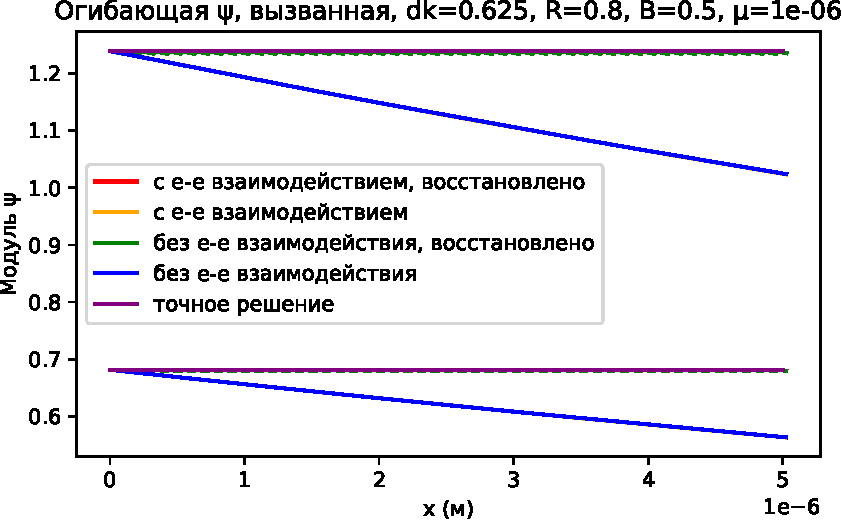
\includegraphics[width=0.4\paperwidth]{figs/error_ru/absEnv2}
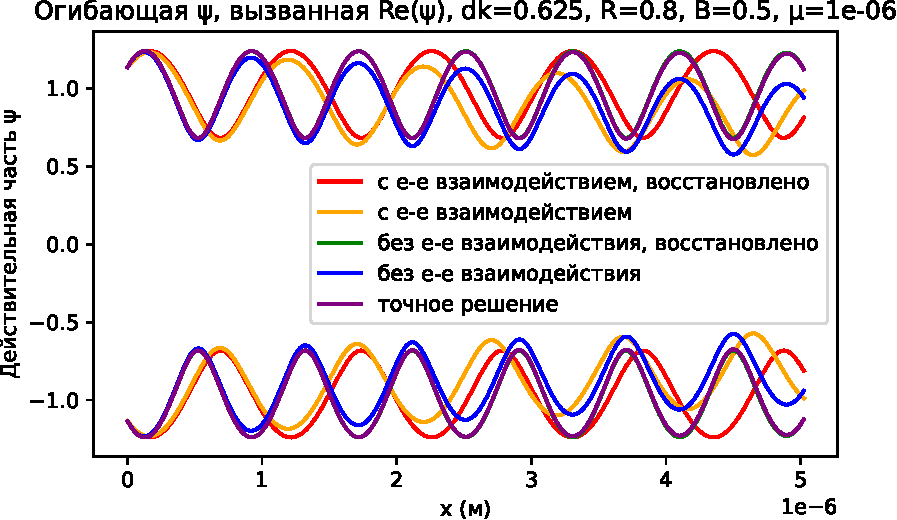
\includegraphics[width=0.4\paperwidth]{figs/error_ru/realEnv2}
\caption{\label{fig:restAmp}
Показанные здесь графики совпадают с верхними графиками на рисунке \ref{fig:linbvp}, показывающими огибающие, соответствующий быстрые колебания решений $\psi$, но с дополнительными кривыми для случаев, когда численное решение имело $\left|\psi\right|$, возвращено к его первоначальному значению каждые 4 колебания $\left|\psi\right|^2$. \\
Цвета кривых следующие: Красная кривая соответствует решению нелинейного уравнения Шредингера с периодически восстанавливаемой амплитудой. Золотая кривая соответствует решению нелинейного уравнения Шредингера без устранения ошибки. Зеленая кривая соответствует решению линейного уравнения Шредингера с периодически восстанавливаемой амплитудой. Синяя кривая соответствует решению этого решения без устранения ошибки. А фиолетовая кривая - это известное точное решение линейного уравнения Шредингера. \\
На левом графике пилообразный рисунок, вызванный периодическим восстановлением амплитуды, приводит к тому, что эти решения слегка видны из-за фиолетовой кривой, в то время как золотая линия полностью скрыта за синей линией. На правом графике зеленая линия скрыта за фиолетовой, но слегка видна при больших значениях $x$.
%The graphs shown here are the same as the top graphs of Figure \ref{fig:linbvp}, showing the envelopes formed by the fast oscillation of the solutions $\psi$, but with additional curves for cases when the numerical solution had $\left|\psi\right|$ returned to its original value every 4 oscillations of $\left|\psi\right|^2$. \\
%The colors of the curves are as follows -- The red curve is for the nonlinear Schrodinger equation with the amplitude periodically restored. The gold curve is for the nonlinear Schrodinger equation without error removal. The green curve is for the linear Schrodinger equation with the amplitude periodically restored. The blue curve is for this solution without error removal. And the purple curve is the known exact solution to the linear Schrodinger equation. \\
%In the left graph, the sawtooth pattern caused by periodically restoring the amplitude causes these solution to be seen slightly from behind the exact case, while the gold line is completely hidden behind the blue line. In the right graph, the green line is hidden behind the purple one, but is slightly visible for larger $x$ values.
}
\end{figure}
\end{center}

Вычисления периода быстрых колебаний показывают постоянное убывание периода, независимо от $\mu$. Одна и та же величина изменения проявляется как в решении линейных, так и в решении нелинейных уравнений -- период постоянно недооценивается. Здесь также присутствует хаотический член, независимый от $\mu$, в то время как ни один из зависимых от $\mu$ членов не демонстрирует такого хаотического поведения, а скорее красиво и чисто расширяется в ряд Тейлора. Таким образом, кажется, что ошибку можно устранить, скорректировав результаты. Вернемся к анализу ошибок периода в разделе \citeph и приложении \citeph .
%Calculations of the fast oscillation period show a constant decrease in period, independent of $\mu$. The same pattern appears in both linear and nonlinear calculations -- we are systematically underestimating the period. There is also a chaotic term here independent of $\mu$, while none of the $\mu$ dependent terms show this chaotic behavior, but rather nicely and cleanly expand into a Taylor series. So it seems that the error is removable by adjusting the results to compensate for the error of the linear solution. We will return to error analysis of the period in Section \citeph and Appendix \citeph . 

Когда амплитуда фиксировано к её начальному значению, можно увидеть ещё результат. Все изменения периодов на расстоянии исчезают, когда амплитуда колебаний $\left|\psi\right|$ устанавливается на её исходное значение. Похоже, что период действительно чувствителен к амплитуде колебаний $\left|\psi\right|$, или, скорее, $\mu$, которая масштабируется на основе $\left|\psi\left(0\right)\right|^ 2$.
%Combining this, one can see another result. All variations of the periods over distance disappear when the amplitude of the $\left|\psi\right|$ oscillations is fixed to its initial value. It seems that the period is indeed sensitive to the amplitude of the $\left|\psi\right|$ oscillations, or rather $\mu$, which rescales based on $\left|\psi\left(0\right)\right|^2$. 

\subsection{Функциональная форма}

Результаты анализа начальной задачи для нелинейного уравнения Шредингера, заданные уравнением \ref{eqn:schrod}, являются решениями вида,
%The results of analysis of the initial value problem with the nonlinear Schrodinger equation given by Equation \ref{eqn:schrod} are solutions of the form,
\begin{equation}
\psi = e^{i M_j x_j} \left( a_j e^{i k_j x_j} + b_j e^{- i k_j x_j} \right),
\end{equation}
которые выглядят как решения линейного уравнения Шредингера,
%which looks like the solutions to the linear Schrodinger equation, 
\begin{equation}
\psi = e^{i M_0 x} \left( a e^{i k_0 x} + b e^{- i k_0 x} \right),
\end{equation}
но волновые числа $k_{\mu}$ и $M_{\mu}$ изменились по сравнению с волновыми числами решения линейного уравнения Шредингера, для которого $M_{0}$ = $\frac{\pi BR}{\Phi_0}$ и $k_{0}$ = $k0 + \frac{dk}{2 R_{max} }$. Эта форма представляется как приближенное решение нелинейного уравнения Шредингера для широкого диапазона разумных значений параметров, в том числе когда $k$ отклоняется от $k_ {Fermi, Au}$. 
На рисунках \ref{fig:beginfo} и \ref{fig:restAmp} показан пример одного из таких решений с параметрами $k = k_{Fermi, Au}$, $R = 8 \times 10^{-7}$ м, $B = 0,5 \, B_{max}$, $\mu = 10^{-6}$ и начальная производная $\psi$, которая решает краевую задачу для линейного уравнения Шредингера. На рисунке \ref{fig:beginfo} показаны быстрые колебания, в то время как на рисунке \ref{fig:restAmp} показана огибающая, образованная быстрыми колебаниями. Приведенная форма для этих решений на самом деле не соответствует требуемому уравнению Шредингера, но это просто означает, что существует отклонение от синусоидальности, как и ожидалось для нелинейных волн.
%but the wave numbers $k_{\mu}$ and $M_{\mu}$ have shifted from those of the solution to the linear Schrodinger equation, for which $M_{0}$ = $\frac{\pi BR}{\Phi_0}$, and $k_{0}$ = $k0 + \frac{dk}{2  R_{max} }$. This form appears as the approximate solution to the ODE for a wide range of reasonable parameter values, including when $k$ deviates from $k_{Fermi, Au}$. 
%Figures \ref{fig:beginfo} and \ref{fig:restAmp} show a sample of one such solution, with the parameters $k = k_{Fermi, Au}$, $R = 8 \times 10^{-7}$, $B = 6.5 \times 10^{-3} \, \mathrm{T}$, $\mu = 10^{-6}$, and an initial $\psi$ derivative which solves the boundary value problem for the linear case. Figure \ref{fig:beginfo} shows the fast oscillations, while Figure \ref{fig:restAmp} shows the envelope formed by the fast oscillations. The given form for these solutions does not actually fit the required Schrodinger equation, but that just means there is a deviation from sinusoidality, as expected for nonlinear waves. 

\subsection{Аналитический анализ}
Поскольку уравнение для анализа является нелинейным, оно лучше всего поддается численному анализу. Найденное таким образом решение нелинейного уравнения Шредингера имеет структуру, аналогичную линейному случаю, но со смещением частоты. Отклонение формы колебаний от синусоидальности слишком мало, чтобы быть заметным.

Аналитический анализ, однако, может дать определенную информацию, если проблема не станет неразрешимой. Наиболее информативный из таких анализов показывает смещение $k$.

%Since the equation for analysis is nonlinear, it is most amenable to numerical analysis. The solution thus found for the ODE shows a similar structure to the linear case, but with a shift in frequency. Departure from sinusoidality of the form of the oscillations is too small to be visible.

%Analytic analysis, however, can provide certain insights, if the problem doesn't become insolvable. The most enlightening of such analyses shows the shift in $k$. 

\subsubsection{Смещение $k$}

Начнем с того, что нелинейное уравнение Шредингера для анализа имеет вид,
%To begin with, the nonlinear Schrodinger equation for analysis is of the form,
\begin{equation}
0 = - \psi^{\prime\prime} + 2 i M_0 \psi^\prime + M_0^2\psi-k_0^2\psi + H_{nl} \left|\psi\right|^2 \psi,
\end{equation}
где $M_0 = \frac{\pi^2 B^2R^2}{\Phi^2_0}$ и $H_{nl} = \mu \frac{m_e}{\left|e\right|\hbar}$. 
Чтобы избавиться от $M_0$, определяем функцию $f$ с помощью,
%To get rid of the $M_0$ term, we define a function $f$ by,
\begin{equation}
\psi \left(x\right) = e^{i M_0 x} f\left(x\right).
\end{equation}
При таком определении дифференциальное уравнение для $f$ имеет вид,
%With this definition, the differential equation for $f$ is,
\begin{equation}
0 = - f^{\prime\prime} - k_0^2 f + H_{nl} \left|f\right|^2 f.
\end{equation}

Теперь проанализируем дифференциальное уравнение, предполагая, что оно близко к линейному, путем последовательных приближений. Начнем с линейного решения и возьмем
%Now we analyze the differential equation, assuming it is close to linearity, by taking successive approximations. We start with the linear solution and take 
\begin{equation}
f_0 = a_0 e^{i k_0 x} + b_0 e^{- i k_0 x},
\end{equation}
известное решение линейного уравнения Шредингера.
Здесь попробуем второе приближение, $f_1 = f_0 + g_1$, где $g_1$ является корректирующим членом. Дифференциальное уравнение для $f_1$ имеет вид,
%the known solution to the linear ODE.
%Here, we will now try a second approximation, $f_1 = f_0 + g_1$, with $g_1$ being the correction term. The differential equation for $f_1$ is,
\begin{equation}
0 = - f_1^{\prime\prime} - k_0^2 f_1  + H_{nl} \left|f_0\right|^2 f,
\end{equation}
где $f$ равно либо $f_1$, если это приведет к линейному уравнению Шредингера, либо $f_0$, если нет. Теперь уравнение можно решить для $\left|f_0\right|^2$,
%where $f$ is either $f_1$ if this would produce a linear ODE, or $f_0$ if not. The equation can now be solved for $\left|f_0\right|^2$,
\begin{equation}
\left|f_0\right|^2 = \left|a_0\right|^2 + \left|b_0\right|^2 + a_0\bar{b}_0e^{2ik_0x}+ \bar{a}_0b_0e^{-2ik_0x}.
\end{equation}
Что здесь интересно, так это то, что член $\left|a_0\right|^ 2 + \left|b_0\right| $ является константой, поэтому для этого члена $f$ можно принять за $f_1$, а не за $f_0$. Полученное уравнение имеет вид
%What is interesting here is that the term of $\left|a_0\right|^2 + \left|b_0\right| $ is a constant, so for this term, $f$ can be taken to be $f_1$, and not $f_0$. The resulting equation is
\begin{equation}
 f_1^{\prime\prime} + k_0^2 f_1  - H_{nl} \left(\left|a_0\right|^2+\left|b_0\right|^2 \right) f = 2 \Re \left( a_0\bar{b}_0e^{2ik_0x} \right)  H_{nl}\left(a_0 e^{i k_0 x} + b_0 e^{- i k_0 x}\right)
\end{equation}
Это уравнение представляет собой консервативным гармоническим осциллятором с волновым числом $k_1 = \sqrt{k_0^2- H_{nl} \left(\left|a_0\right|^2+\left|b_0\right|^2 \right)}$, испытывающим вынужденные колебания с волновыми числами из $k_0$ и $3k_0$.
%This equation is a driven harmonic oscillator with a wave number of  $k_1 = \sqrt{k_0^2- H_{nl} \left(\left|a_0\right|^2+\left|b_0\right|^2 \right)}$, driven by oscillations with wave numbers of $k_0$ and $3k_0$. 

Учитывая, что $f_0\left(0\right) = a_0 + b_0$ и $f^\prime_0\left(0\right) = ik_0 \left(a_0-b_0\right)$, $\left|a_0\right|^2+\left|b_0\right|^2$ можно переписать следующим образом,
%Given that $f_0\left(0\right) = a_0 + b_0$ and $f^\prime_0\left(0\right) = ik_0 \left(a_0-b_0\right)$ The term $\left|a_0\right|^2+\left|b_0\right|^2$ can be rewritten as,
\begin{equation}
\left|a_0\right|^2 +\left|b_0\right|^2 = \frac{1}{2}\left(
\left|f_0\left(0\right)\right|^2 + \frac{\left|f^\prime_0\left(0\right)\right|^2}{k^2_0}
\right).
\end{equation} 
Теперь можно определить волновую функцию, соответствующую $f_0$, как
%One can now define the wave function which corresponds to $f_0$ as
\begin{equation}
\psi_0 = e^{i M_0 x} \left( a_0 e^{i k_0 x} + b_0 e^{- i k_0 x} \right),
\end{equation}
с производной при $x = 0$
%with a derivative at $x = 0$ of
\begin{equation}
\psi_0^\prime\left(x\right) = i M_0 + i k_0 \left( a_0 - b_0 \right) = i M_0 + f_0^\prime.
\end{equation}
Это означает, что
%This means that 
\begin{equation}
\left|a_0\right|^2 +\left|b_0\right|^2 = \frac{1}{2}\left(
\left|\psi_0\left(0\right)\right|^2 + \frac{\left|\psi^\prime_0\left(0\right)\right|^2}{k^2_0} - 3M_0^2 + 2 M_0 \Im \left(\frac{\psi^\prime_0}{k_0}\right)
\right).
\end{equation} 
Первые два из этих членов соответствуют основной поправке к $k$, найденной численно в главе \citeph .
%The first two of these terms correspond to the main correction to $k$ found numerically in the Chapter \citeph .

%\subsubsection{Shift in $M$}
%I start this analysis with the assumption that the wave function of analysis can be defined as the product of two periodic functions,
%\begin{equation}
%\psi_j\left(x\right) = f\left(x\right) g\left(x\right),
%\end{equation}
%where $f_j\left(x\right)$ is periodic, with period $k_j$ and $g_j\left(x\right)$ is periodic with period $M_j$, with $k_j \ggg g_j$. Furthermore, $\left|g_j\left(x\right)\right|$ is a constant, i.e. the function $g_j$ is a phase shift which leaves the amplitude of the overall function constant, 
%\begin{equation}
%g_j\left(x\right) = e^{i h_j\left(x\right)},
%\end{equation}
%where $h_j$ is a real function of $x$. In order to remove the function $f_j$, we sample $\psi_j$ in intervals of $\frac{2 \pi}{k_j}$, and examine the equations for the resulting function. Therefore, $f_j$, $f_j^\prime$, and $f_j^{\prime\prime}$ are three unknown constants. If I choose to start sampling at $x=0$, I can find these constants based on my known initial values for $\psi_j$, as $\psi_j\left(0\right) = f\left(0\right) g\left(0\right)$. I define $g\left(0\right) = 1$, and thus $f\left(0\right) = \psi_j\left(0\right) = 1$.  
%
%\begin{equation}
%\psi_j^\prime = f^\prime g + f g^\prime,
%\end{equation}
%\begin{align}
%\psi_j^{\prime\prime} &= f^{\prime\prime} g + f g^{\prime\prime} + 2 f^\prime g^\prime \\&= 2 i M_0 \psi^\prime + M^2\psi-k^2\psi + H_{nl} \left|\psi\right|^2 \psi \\&= 2 i M_0 f^\prime g + 2 i M_0 f g^\prime + M^2 f g - k^2 f g + H_{nl} \left|f\right|^2 f g,
%\end{align}
%\begin{equation}
%0 = - f g^{\prime\prime} + \left( 2 f^\prime + 2 i M_0 f \right) g^\prime - \left( f^{\prime\prime} + 2 i M_0 f^\prime   + M^2 f  - k^2 f  + H_{nl} \left|f\right|^2 f \right) g,
%\end{equation}
%This can be rewritten with equation x
%\begin{equation}
%0 = - f g \left(- (h^\prime)^2 + i h^{\prime\prime} \right) + \left( 2 f^\prime + 2 i M_0 f \right) i h^\prime g - \left( f^{\prime\prime} + 2 i M_0 f^\prime   + M^2 f  - k^2 f  + H_{nl} \left|f\right|^2 f \right) g,
%\end{equation}
%we can now divide by $fg$
%\begin{equation}
%0 = -  \left(- (h^\prime)^2 + i h^{\prime\prime} \right) + \left( 2 \frac{f^\prime}{f} + 2 i M_0  \right) i h^\prime  - \left( \frac{f^{\prime\prime}}{f} + 2 i M_0 \frac{f^\prime}{f}   + M^2   - k^2   + H_{nl} \left|f\right|^2  \right) ,
%\end{equation}
%This equation can now be split into real and imaginary components. The real component is as follows
%\begin{equation}
%0 =  (h^\prime)^2 + \left( -2\, \Im\left(\frac{f^\prime}{f}\right) - 2 M_0  \right) h^\prime  - \left(\Re\left( \frac{f^{\prime\prime}}{f}\right)  + M^2   - k^2   + H_{nl} \left|f\right|^2  \right) ,
%\end{equation}
%%The other term linear in $\mu$ which appears there (a $\mu\frac{M}{k}\Im \left(\psi^\prime\left(0\right)\right)$ term) corresponds to the shift in $M$. 
%While equation x looks like a big mess, everything except $h^\prime$ is just a number, so the solutions must have $h^\prime$ equal to some constant. 
%\begin{equation}
%h^\prime = M = \Im\left(\frac{f^\prime}{f}\right) + M_0 \pm \sqrt{\left(\Im\left(\frac{f^\prime}{f}\right) + M_0\right)^2 +\Re\left( \frac{f^{\prime\prime}}{f}\right)  + M^2   - k^2   + H_{nl} \left|f\right|^2}
%\end{equation}
%%\left(\Im\left(\frac{f^\prime}{f}\right) + M_0\right)^2 + \Re\left( \frac{f^{\prime\prime}}{f}\right)  + M^2   - k^2   + H_{nl} \left|f\right|^2}}
%\begin{equation}
%h^\prime = \Im\left(\frac{f^\prime}{f}\right) + M_0 \pm \sqrt{\left(\Im\left(\frac{f^\prime}{f}\right) + M_0\right)^2 + k^2  + M_0^2   - k_0^2   + H_{nl} }
%\end{equation}

\end{document}


















